\newpage

\lecture{10}{20 Nov. 14:20}{}

\begin{figure}[H]
    \centering
    \begin{tikzpicture}[
        >=Stealth,
        node distance=1.8cm and 1.8cm,
        every node/.style={font=\small},
        v/.style={circle, draw, thick, minimum size=8mm},
        edge/.style={->, thick}
    ]
        % nodes
        \node[v, fill=gray!15] (s) {$s$};
        \node[v, right=1.5cm of s] (a) {$u_1$};
        \node[v, below=1.2cm of a] (b) {$u_2$};
        \node[v, right=1.5cm of a] (c) {$v_1$};
        \node[v, below=1.2cm of c] (d) {$v_2$};
        \node[v, fill=gray!15, right=1.5cm of c] (t) {$t$};
    
        % edges with flow/capacity
        \draw[edge] (s) -- (a) node[midway, above] {$\;3/\textcolor{red}{10}$};
        \draw[edge] (s) -- (b) node[midway, below, sloped]  {$\;2/\textcolor{red}{8}$};
        \draw[edge] (a) -- (c) node[midway, above] {$\;2/\textcolor{red}{5}$};
        \draw[edge] (a) -- (d) node[midway, sloped, above] {$\;1/\textcolor{red}{4}$};
        \draw[edge] (b) -- (d) node[midway, below] {$\;2/\textcolor{red}{7}$};
        \draw[edge] (c) -- (t) node[midway, above] {$\;2/\textcolor{red}{6}$};
        \draw[edge] (d) -- (t) node[midway, below, sloped] {$\;3/\textcolor{red}{9}$};
    \end{tikzpicture}
    \caption{Example of Maxflow Problem}
\end{figure}

考慮 Ford-Fulkerson algorithm 的複雜度分析,如果所有容量都是整數,則每次增廣至少增加 1 單位的流量,而 $m$ 條管線的容量總和是 $C = \sum_{e \in E} c(e)$,因此最多增廣 $C$ 次,每次找增廣路徑花費$O(m)$的時間,總複雜度是 \[
    T(m, C) = O(C) \cdot O(m) = O(mC)
\]
但,這個算是「多項式時間」(polynomial time)演算法嗎?還是是「指數時間」(exponential time)演算法?
\begin{remark}
    Complexity is according to the input size of an instance.
\end{remark}

\begin{eg}
    For an $n \times n$ matrix multiplication problem, the input size is $N = \Theta(n^2)$ (set all the number is of size $O(1)$).
\end{eg}

The complexity is 
\begin{itemize}
    \item Linear-time if $T(N) = O(N) = O(n^2)$.
    \item Polynomial-time if $T(N) = O(N)^{O(1)} = O(n)^{O(1)}$.
    \item Exponential-time if $T(N) = O(1)^N = O(1)^{n^2}$ or more.
\end{itemize}

\begin{definition}[Complexity of Linear/Quadratic/Polynomial-time Algorithms]
For any instance $I$,define its input size as a non-negative integer function
\[
    N = \mathrm{size}(I),
\]
其中 $N$ 表示描述輸入實例所需的位元數或其他適當的度量方式。
令 $T(N)$ 為某演算法在輸入大小為 $N$ 時的最壞情況執行時間。我們對時間複雜度作如下分類:
\begin{itemize}
    \item Linear-time algorithm:若 $T(N) = O(N)$。
    \item Quadratic-time algorithm:若 $T(N) = O(N^2)$。
    \item Polynomial-time algorithm:若存在常數 $k$ 使得 $T(N) = O(N)^{O(1)}$。
    \item Exponential-time algorithm:若存在常數 $c > 1$ 使得 $T(N) = O(1)^N$ or more。
\end{itemize}
\end{definition}

\newpage

\begin{eg}
    For a prime testing problem, given an integer $N$ as input.
\end{eg}

We have to consider the input size.
\begin{itemize}
    \item If input size is $N = O(1)$, then the method of checking all integers from $2$ to $\sqrt{N}$ is \[
        O(\sqrt{N}) = O(1)
    \] which is a linear-time algorithm.
    \item If the size of $N$ is not constrainted, then the input size is $\Theta(\log N)$ (bits to represent $N$). The time of checking all integers from $2$ to $\lfloor \sqrt{N} \rfloor$ is $\Omega(\sqrt{N})$
    \begin{itemize}
        \item According to \[
            (\log N)^{O(1)} = o(\sqrt{N}) = o(N^{1/2})
        \]
        this algorithm is not polynomial-time.
        \item According to \[
            O(N^{1/2}) = O(1)^{O(\log N)}
        \]
        this algorithm is singly exponential-time.
    \end{itemize}
\end{itemize}

\begin{note}
    所以根據 maximum flow problem 的 input size 是
    \begin{itemize}
        \item 若 $C = O(1)$,input size 是 $O(m) \cdot O(1) = O(m)$,所需要花的時間是 $O(mC) = O(m)$,演算法是 linear-time。
        \item 若無大小限制,input size 是 $O(m) \cdot O(\log C) = O(m \log C)$,所需要花的時間是 \[
            O(mC) \neq O(m \log C)^{O(1)}
        \]因此演算法不是 polynomial-time。
    \end{itemize}
\end{note}

\begin{remark}
    Ford-Fulkerson algorithm 還會出現無限迴圈的問題,例如下圖的圖,設計出非整數的容量,會導致無限迴圈。Ford-Fulkerson 的論文就有提出其他反例。
    \begin{figure}[H]
        \centering
        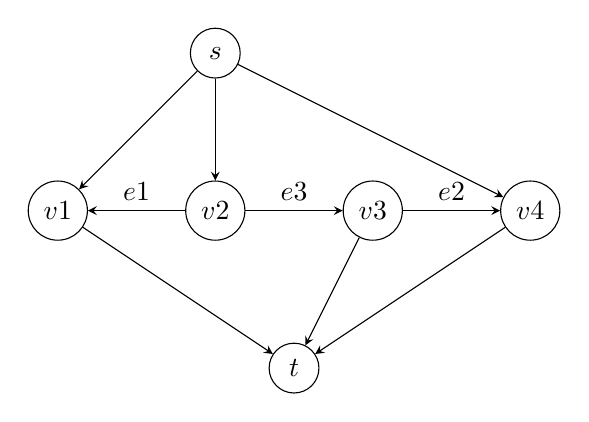
\begin{tikzpicture}[>=stealth, node distance=2cm]

        % nodes
        \node[circle, draw, minimum size=18pt] (s) at (0,2) {$s$};
        \node[circle, draw, minimum size=18pt] (v1) at (-2,0) {$v1$};
        \node[circle, draw, minimum size=18pt] (v2) at (0,0) {$v2$};
        \node[circle, draw, minimum size=18pt] (v3) at (2,0) {$v3$};
        \node[circle, draw, minimum size=18pt] (v4) at (4,0) {$v4$};
        \node[circle, draw, minimum size=18pt] (t) at (1,-2) {$t$};

        % edges from s
        \draw[->] (s) -- (v1);
        \draw[->] (s) -- (v2);
        \draw[->] (s) -- (v4);

        % edges v2 -> v1 (e1)
        \draw[->] (v2) -- node[above] {$e1$} (v1);

        % edges v3 -> v4 (e2)
        \draw[<-] (v4) -- node[above] {$e2$} (v3);

        % edges v2 -> v3 (e3)
        \draw[->] (v2) -- node[above] {$e3$} (v3);

        % edges to t
        \draw[->] (v1) -- (t);
        \draw[->] (v3) -- (t);
        \draw[->] (v4) -- (t);

        \end{tikzpicture}
        \caption{A graph that may cause infinite loop in Ford-Fulkerson algorithm}        
    \end{figure}
\end{remark}

\newpage

\section{Edmonds-Karp Algorithm}
這是史上第一個被證明是 polynomial-time 的 maximum flow algorithm。

\begin{theorem}
    If one make sure that the augmenting $st$-path in $R(f)$ is always the shortest path from $s$ to $t$ (in terms of number of edges), then the Ford-Fulkerson algorithm runs in $O(m^2 n)$ time.
\end{theorem}

\begin{com}[1]
    在保證每次 augmenting path 都是 shortest path 的前提下,Edmonds-Karp algorithm 保證在 $mn$ round 內結束。
\end{com}

\begin{com}
    無需假設 $G$ 所有容量都是整數。
\end{com}

We need two lemmas to prove the above theorem.

\begin{notation}
    $d_f^*(s, u)$ is the shortest distance from $s$ to $u$ in unweighted version of $R(f)$.
\end{notation}

\begin{lemma}[現邊觀察]
    If in $R(f+g)$ exists $uv$ edge which is not in $R(f)$, then \[
        d_{R(f+g)}^*(s, u) = d_{R(f)}^*(s, v) + 1
    \]
\end{lemma}
\begin{proof}
    Let $P$ be the shortest augmenting $st$-path of $R(f)$. If $R(f)$ don't have the $uv$ edge, $P$ can't go through $uv$ edge. If it does not go through $vu$ edge, too. Then $g(uv) = g(vu) = 0$. We get
    \begin{align*}
        (f+g)(uv) &= f(uv) + g(uv) - g(vu) = f(uv) \\
        (f+g)(vu) &= f(vu) + g(vu) - g(uv) = f(vu)
    \end{align*}
    Then we get $R(f+g) = R(f)$ which can not have $uv$ edge, which is contradiction. So $P$ must go through $vu$ edge. Then we have \[
        d_{f+g}^*(s, u) = d_f^*(s, v) + 1
    \]
    Proof complete.
\end{proof}

\begin{lemma}[遞增觀察]
    Let $P$ be the shortest augmenting $st$-path of $R(f)$. Let $g$ be the saturating flow for $R(f)$ correspond to $P$. Then for any $v \in V(G)$ we have \[
        d_{R(f+g)}^*(s, v) \geq d_{R(f)}^*(s, v)
    \]
\end{lemma}
\begin{proof}
    Assume for contradiction that there exists some $v \in V(G)$ such that \[
        d_{R(f+g)}^*(s, v) < d_{R(f)}^*(s, v) \tag{1}
    \]
    Thus, $d_{f+g}^*(s, v) \neq \infty$. Let $v$ be such vertex with the smallest $d_{f+g}^*(s, v)$. We know $v \neq s$ since $d_{f+g}^*(s, s) = d_f^*(s, s) = 0$. Let $Q$ be the unweighted shortest $sv$-path in $R(f+g)$ ($u$ could be $s$). Let $uv$ be the last edge of $Q$. We have \[
        d_{R(f)}^*(s, u) \leq d_{R(f+g)}^*(s, u) \tag{2}
    \]
    If \blue{$uv \subseteq R(f)$}, then equation \red{(2)}, and \yel{$uv \in Q$} imply \[
        d_{R(f)}^*(s, v)\ \blue{\leq}\ d_{R(f)}^*(s, u) + 1\ \red{\leq}\ d_{R(f+g)}^*(s, u) + 1\ \yel{=}\ d_{R(f+g)}^*(s, v)
    \]
    which is contradiction to equation (1). \\
    If $uv \not\subseteq R(f)$, by \blue{現邊觀察} ($uv \not\subseteq R(f)$ and $uv \subseteq Q \subseteq R(f+g)$), then equation \red{(2)} and \yel{$uv \subseteq Q$} imply \[
        d_{R(f)}^*(s, v)\ \blue{=}\ d_{R(f)}^*(s, u) - 1\ \red{\leq}\ d_{R(f+g)}^*(s, u) - 1\ \yel{=}\ d_{R(f+g)}^*(s, v) - 2 
    \]
    which is contradiction to equation (1), too.
\end{proof}

\vspace{1em}

Now let compute the time complexity of Edmonds-Karp algorithm.

\vspace{1em}

\begin{proof}[Time Complexity]
    Since each augmenting path can be found by BFS in $O(m)$ time, we only need to proof that algorithm halt in $O(mn)$ rounds. 

    \begin{claim}
        Every round ``saturates'' at least one edge in the shortest $st$-path $P$ found in that round, which is $O(m)$ edges in $G \cup G^r$, causing them to be removed from the residual graph of the next round. Thus, we can just show that each $uv \subseteq G \cup G^r$ being removed $O(n)$ times in total.
    \end{claim}

    Suppose that an edge $uv$ of $G \cup G^r$ is not in $R(f)$
    \begin{itemize}
        \item appears in $R(f + g)$ and 
        \item removed in $R(f + g + \cdots + g' + h)$ for the first time after $R(f + g)$
    \end{itemize}
    where $h$ is the saturating flow of $R(f + g + \cdots + g' + h)$ corresponding to the shortest augmenting $st$-path in $R(f + g + \cdots + g')$ saturates $uv$. Thus, $uv \in E(P)$. We have 
    \begin{align*}
        d_{R(f)}^*(s, u) &= d_{R(f)}^*(s, v) + 1 \quad &\text{by 現邊觀察} \\
        &\leq d_{R(f + g + \cdots + g')}^*(s, v) + 1 \quad &\text{by 遞增觀察} \\
        &= d_{R(f + g + \cdots + g' + h)}^*(s, u) + 2 \quad &uv \in E(P)
    \end{align*}
    Since $d_H^*(s, u) \in \{0, 1, \cdots, n-1, \infty\}$ for any residual graph $H$, $uv$ can at most appear and disappear $O(n)$ times in the residual graphs throughout the algorithm. Thus, the algorithm halts in $O(mn)$ rounds. and thus run in $O(m^2 n)$ time.
\end{proof}

\noindent\rule{\textwidth}{0.4pt}

Edmonds-Karp 的分析是用邊來看:
\begin{itemize}
    \item 每條邊 $uv$ 只要「出現之後消失」一次,就會讓 $d_R^*(s, u)$ 增加,
    \item 每個節點 $u$ 的 $d_R^*(s, u)$ 只有 $O(n)$ 個可能的值.
\end{itemize}
所以每個邊「出現之後消失」$O(n)$ 次,每回合至少消失一條邊,一共 $O(mn)$ 回合。如果用節點 $u$ 來看,能不能根據一樣的證明,得知
\begin{itemize}
    \item 節點 $u$ 的任一 outgoing edge「出現之後消失」一次,則 $d_R^*(s, u)$ 的值會增加,
    \item 節點 $u$ 的 $d_R^*(s, u)$ 只有 $O(n)$ 個可能的值,
\end{itemize}

所以 $u$ 的所有 outgoing edges 全部只能「出現之後消失」$O(n)$ 次,而每回至少讓一條邊消失,所以總共只有 $O(n^2)$ 回合?

\noindent\rule{\textwidth}{0.4pt}

答案是錯誤的,
\begin{quote}
    因為節點 $u$ 的任一 outgoing edge『出現之後消失』一次,則 $d_{R(f)}^*(s, u)$ 的值會增加至少 2
\end{quote}
是錯的,邊消失一次,$d_{R(f)}^*(s, u)$ 不一定會增加,因為可能有其他替代路徑,不一定是 shortest path

\newpage

\section{Bipartite Matching via Maximum Flow}

\begin{problem}[Maximum matching of bipartite graph]
    Given
    \begin{itemize}
        \item Input: An undirected ``bipartite'' graph $G$
        \item Output: A matching $M \subseteq E(G)$ with maximum $|M|$.
    \end{itemize}
\end{problem}

\begin{definition}[Bipartite Graph]
    A graph $G$ is \textbf{bipartite} if there are disjoint vertex subsets $U, V$ of $G$ with $U \cup V = V(G)$ such that every edge of $G$ has one endpoint in $U$ and the other in $V$. 
\end{definition}

\begin{definition}[matching]
    A edge subset $M \subseteq E(G)$ is a \textbf{matching} of $G$ if $M = \emptyset$ or the minimal subgraph $H$ of $G$ with $E(H) = M$ which has $\displaystyle \max_{e \in E(H)} \deg(H) = 1$. 
\end{definition}

\vspace{1em}

We can reduce the maximum matching problem of bipartite graph to the maximum flow problem by the below construction.

Let $G(s, t)$ be the unit-capacity graph obtained from $G$ by adding 
\begin{itemize}
    \item new source vertex $s$ with edges $su$ for all $u \in U$
    \item new sink vertex $t$ with edges $vt$ for all $v \in V$
\end{itemize}

\begin{obs}
    $G$ has a maximum matching with $k$ edges if and only if $G(s, t)$ has a maximum flow with value $k$.
\end{obs}

We separately prove the two directions.
\begin{itemize}
    \item ($\Rightarrow$) Let $M$ be a maximum matching of $G$ we have to make sure it follow capacity constraints and Conservation law.
    \begin{itemize}
        \item Capacity constraints: 因為是一對一 matching,所以每個 $u \in U$ 和 $v \in V$ 最多只有一條 flow 1 的邊經過。
        \item Conservation law: For each vertex $u \in U$, at most one edge $su$ has flow 1, and for each vertex $v \in V$, at most one edge $vt$ has flow 1, and for each $uv \in M$, at most exists one flow from $U \to V$.
    \end{itemize}
    \item ($\Leftarrow$) Define $M = \{uv \in E(G) : f(uv) = 1\}$. We have to make sure $M$ is a matching. And by the proposition below, $|M| = k$.
\end{itemize}
\begin{proposition}
    If $G(s, t)$ has a maximum flow with value $k$, then $G(s, t)$ has an ``integral'' flow with value $k$. Given that each edge of $G(s, t)$ has unit capacity, the set of edges in the middle part of $G(s, t)$ with non-zero flow forms a matching of $G$ with $k$ edges. Due to $f$ is closed under $\{+, -\}$.
\end{proposition}

\chapter{Computational Geometry}
\section{Nearest Point Pair}

\begin{problem}[Nearest Point Pair Problem]
    Given
    \begin{itemize}
        \item Input: A set $P$ of $n$ points in the plane.
        \item Output: A pair of points $p, q \in P$ such that the Euclidean distance $d(p, q)$ is minimized.
    \end{itemize}
\end{problem}

\begin{com}
    Not losing generality, we can assume that \[
        |P| = 2^k, \quad k \in \mathbb{N}
    \]
\end{com}

\vspace{1em}

A naive algorithm is to compute the distance of each pair of points, then solve a 老大問題,which takes $O(n^2)$ time.

\begin{figure}[H]
    \centering
    \begin{tikzpicture}[dot/.style={circle, fill=gray!60, minimum size=6pt, inner sep=0pt}]
        % --- Left side label L ---
        \node at (-4, 3.5) {\Large\itshape L};
    
        % --- Right side label R ---
        \node at (4, 3.5) {\Large\itshape R};
    
        % --- Vertical dividing line ---
        \draw[very thin, red!40] (0, -2) -- (0, 4);
    
        % --- Left-side nodes (manual placement to match scattered layout) ---
        \node[dot] (l1) at (-3.2, 2.5) {};
        \node[dot] (l2) at (-2.3, 1.4) {};
        \node[dot] (l3) at (-3.7, 0.6) {};
        \node[dot] (l4) at (-2.5, -0.2) {};
        \node[dot] (l5) at (-3.0, -1.4) {};
        \node[dot] (l6) at (-1.2, 2.6) {};
        \node[dot] (l7) at (-0.8, 1.0) {};
    
        % --- Right-side nodes ---
        \node[dot] (r1) at (3.0, 2.6) {};
        \node[dot] (r2) at (2.2, 1.7) {};
        \node[dot] (r3) at (3.4, 0.8) {};
        \node[dot] (r4) at (2.4, -0.3) {};
        \node[dot] (r5) at (3.5, -1.2) {};
        \node[dot] (r6) at (1.5, 2.4) {};
        \node[dot] (r7) at (0.5, -1.0) {};
    \end{tikzpicture}
    \caption{Divide-and-Conquer Strategy for Nearest Point Pair Problem}
\end{figure}

We can use divide-and-conquer strategy to solve this problem follow the above graph.

\newpage

\begin{idea}
    Pre sort $P$ by $y$-coordinate as $P_y$, which would take 
    \[
        O(n \log n)
    \]
    Then, use divide-and-conquer strategy to solve the problem
    \begin{enumerate}[label=$\arabic*^\circ$]
        \item Spend $O(n)$ time to split $P$ into two halves $P_L$ and $P_R$, \[
            P_L = \{p \mid p \in P : x(p) \leq x_{\text{mid}}\}, \quad P_R = \{p \mid p \in P : x(p) > x_{\text{mid}}\}
        \]
        with $x_{\text{mid}}$ being the median $x$-coordinate of points in $P$. We can use the minimum-selection algorithm to find the median in $O(n)$ time.
        \item Output a closest pair among the following three pairs:
        \begin{itemize}
            \item The closest pair in $P_L$ (recursively solved).
            \item The closest pair in $P_R$ (recursively solved).
            \item The closest pair $(p, q)$ with $p \in P_L$ and $q \in P_R$, which can be solved in $O(n)$ time as below.
        \end{itemize}
        \begin{note}
            Follow the graph below, the node will exist in the vertical strip with width $2d$ centered at the dividing line. For each point $p$ in the strip, we only need to check at most 8 points in the box. So the complexity is $$O(n) \times O(1) = O(n)$$
        \end{note}
    \end{enumerate}
\end{idea}

\vspace{1em}

\begin{figure}[H]
    \centering
    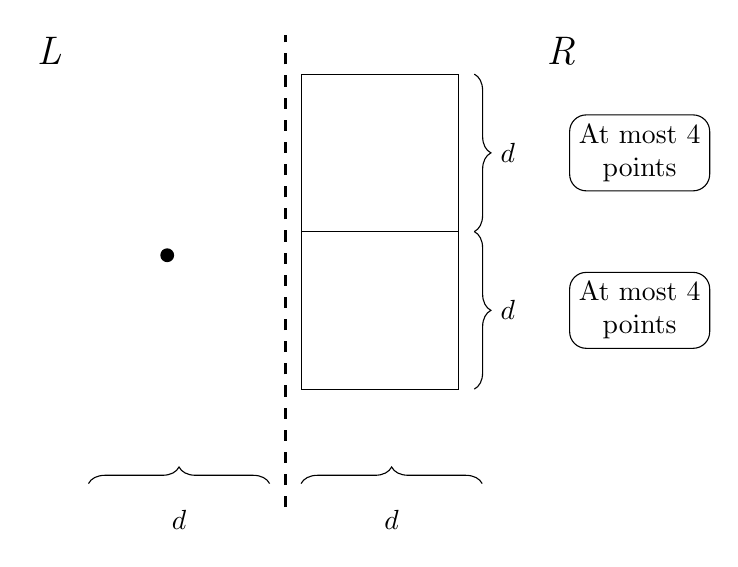
\begin{tikzpicture}[
        dot/.style={circle, fill=black, minimum size=5pt, inner sep=0pt},
        rect/.style={draw, fill=white},
    ]
    % Move the whole figure upward slightly for vertical centering
    \begin{scope}[yshift=0cm]
    % Labels L, R
    \node at (-3, 2.8) {\Large\itshape L};
    \node at ( 3.5, 2.8) {\Large\itshape R};
    
    % Dashed vertical line
    \draw[line width=1pt, dash pattern=on 4pt off 4pt] (0, -3) -- (0, 3);
    
    % Left lone point
    \node[dot] at (-1.5, 0.2) {};
    
    % Horizontal distance labels (d)
    \draw[decorate,decoration={brace,amplitude=6pt}] (-2.5, -2.7) -- (-0.2, -2.7) node[midway,below=6pt] {$d$};
    \draw[decorate,decoration={brace,amplitude=6pt}] (0.2, -2.7) -- (2.5, -2.7) node[midway,below=6pt] {$d$};
    
    % Vertical rectangles on right side (centered)
    \draw[rect] (0.2, 0.5) rectangle (2.2, 2.5);
    \draw[rect] (0.2, -1.5) rectangle (2.2, 0.5);
    
    % Vertical braces for the two rectangles
    \draw[decorate,decoration={brace,amplitude=6pt}] (2.4, 2.5) -- (2.4, 0.5) node[midway,right=6pt] {$d$};
    \draw[decorate,decoration={brace,amplitude=6pt}] (2.4, 0.5) -- (2.4, -1.5) node[midway,right=6pt] {$d$};
    
    % Text boxes "At most 4 points"
    \node[draw, fill=white, align=center, rounded corners=6pt] at (4.5, 1.5) {At most 4\\points};
    \node[draw, fill=white, align=center, rounded corners=6pt] at (4.5, -0.5) {At most 4\\points};
    
    \end{scope}
    
    \end{tikzpicture}
    \caption{Finding Closest Pair Across the Dividing Line}
\end{figure}

把所有距離分割線不超過 $d$ 的點挑出來,根據演算法一開始的準備動作,我們只要花 $O(n)$ 時間就可以把這些點根據它們的 $y$ 座標排好。我們稱這個 sorted list 為 $M^*$。
\begin{itemize}
    \item $M^*$ 裡面在 $L$ 中的點的形成 $L^*$, 在 $R$ 中的點形成 $R^*$.
\end{itemize}
再花 $O(n)$ 時間就能夠整理出資料結構使得每個點 $p \in M^*$ 都能在 $O(1)$ 時間查得:
\begin{itemize}
    \item 在 $L^*$ 中 $y$ 座標與 $p$ 的 $y$ 座標最近的上下(按照 $M^*$ 的順序)各一個節點。
    \item 在 $R^*$ 中 $y$ 座標與 $p$ 的 $y$ 座標最近的上下(按照 $M^*$ 的順序)各一個節點。
\end{itemize}
For each point $p$ in $L^*$,
\begin{itemize}
    \item check four points of $R^*$ above $p$ in $M^*$.
    \item check four points of $R^*$ below $p$ in $M^*$.
\end{itemize}
只需要在 $M^*$ 中由上而下走過每個點,每個點在 $M^*$ 的順序中上下各取八個點一定會找到在對面那一側的 $2d \times d$ 的方格內跟自己最近的點(如果格子內有點的話)。

\begin{note}
    By master theorem, the time complexity of this divide-and-conquer algorithm is \[
        T(n) = 2T\left(\frac{n}{2}\right) + O(n)
    \] which gives \[
        T(n) = O(n \log n)
    \] Therefore, the overall time complexity including the initial sorting step is \[
        O(n \log n) + O(n \log n) = O(n \log n)
    \]
\end{note}

\section{Convex Hull}

\begin{problem}[Convex Hull]
    Given 
    \begin{itemize}
        \item Input: A set $P$ of $n$ points in the plane.
        \item Output: The convex polygon with a minimum perimeter enclosing all points in $P$.
    \end{itemize}
\end{problem}

\begin{figure}[H]
    \centering
    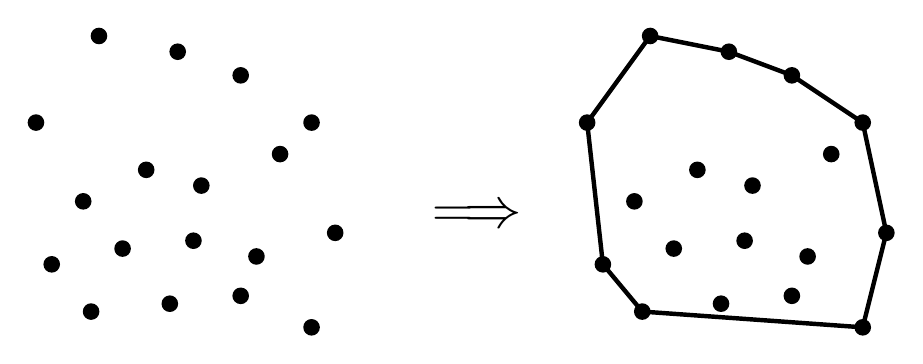
\begin{tikzpicture}[
        dot/.style={circle, fill=black, minimum size=6pt, inner sep=0pt},
        thickline/.style={line width=1.6pt}
    ]

    \begin{scope}[xshift=-3.5cm]
        \node[dot] at (-1.6,1.2) {};
        \node[dot] at (-0.8,2.3) {};
        \node[dot] at (0.2,2.1) {};
        \node[dot] at (1.0,1.8) {};
        \node[dot] at (1.9,1.2) {};
    
        \node[dot] at (-1.0,0.2) {};
        \node[dot] at (-0.2,0.6) {};
        \node[dot] at (0.5,0.4) {};
        \node[dot] at (1.5,0.8) {};
    
        \node[dot] at (-1.4,-0.6) {};
        \node[dot] at (-0.5,-0.4) {};
        \node[dot] at (0.4,-0.3) {};
        \node[dot] at (1.2,-0.5) {};
        \node[dot] at (2.2,-0.2) {};
    
        \node[dot] at (-0.9,-1.2) {};
        \node[dot] at (0.1,-1.1) {};
        \node[dot] at (1.0,-1.0) {};
        \node[dot] at (1.9,-1.4) {};
    \end{scope}
    
    \node at (0.5,0) {\huge $\Longrightarrow$};

    \begin{scope}[xshift=3.5cm]
        \coordinate (p1) at (-1.6,1.2);
        \coordinate (p2) at (-0.8,2.3);
        \coordinate (p3) at (0.2,2.1);
        \coordinate (p4) at (1.0,1.8);
        \coordinate (p5) at (1.9,1.2);
    
        \coordinate (p6) at (-1.0,0.2);
        \coordinate (p7) at (-0.2,0.6);
        \coordinate (p8) at (0.5,0.4);
        \coordinate (p9) at (1.5,0.8);
    
        \coordinate (p10) at (-1.4,-0.6);
        \coordinate (p11) at (-0.5,-0.4);
        \coordinate (p12) at (0.4,-0.3);
        \coordinate (p13) at (1.2,-0.5);
        \coordinate (p14) at (2.2,-0.2);
    
        \coordinate (p15) at (-0.9,-1.2);
        \coordinate (p16) at (0.1,-1.1);
        \coordinate (p17) at (1.0,-1.0);
        \coordinate (p18) at (1.9,-1.4);
    
        \draw[thickline]
            (p2) -- (p3) -- (p4) -- (p5) -- (p14) -- (p18) -- (p15) -- (p10) -- (p1) -- cycle;
    
        \foreach \p in {p1,p2,p3,p4,p5,p6,p7,p8,p9,p10,p11,p12,p13,p14,p15,p16,p17,p18}
            \node[dot] at (\p) {};
            
    \end{scope}
    \end{tikzpicture}
    \caption{Convex Hull Example}
\end{figure}

A naive algorithm is to check the $p \in P$ with minimum $x$-coordinate, which must be a vertex on the convex hull. Then, chose the next vertex with maximum slope to the current vertex. Then, rotate the whole graph until we return to the starting vertex. This algorithm takes $O(n^2)$ time.

\begin{idea}
    Now we introduce a new method with $O(n \log n)$ time complexity.
    \begin{enumerate}[label=$\arabic*^\circ$]
        \item Find the point $p^*$ with the lowest $x$-coordinate in $O(n)$ time (老大問題)
        \item Sort all the points in $P$ by the slope of the line segment $p^* p$ for each $p \in P \setminus \{p^*\}$ in $O(n \log n)$ time.
        \item Chose the initial convex hull $H$ to be the triangle formed by $p^*$ and the first two points in the sorted list.
        \item For each remaining point $p$ in the sorted list, do:
        \begin{itemize}
            \item Beacuse the one we chose the points based on the slope from $p^*$, the point $p$ must be outside the current convex hull $H$.
            \item Move along the boundary of $H$ in clockwise direction from the initial point, and remove all vertices $q$ of $H$ such that the line segment $qp$ makes a left turn with respect to the edge of $H$ incident to $q$.
            \item Do this until we reach a vertex $r$ of $H$ such that the line segment $rp$ makes a right turn with respect to the edge of $H$ incident to $r$.
            \item Add the edge $rp^*$ and $p^* p$ to $H$ to form the new convex hull.
        \end{itemize}
        This step takes $O(n)$ time in total because each point is added and removed at most once.
    \end{enumerate}
    Therefore, the overall time complexity is \[
        O(n) + O(n \log n) + O(n) = O(n \log n) 
    \] \hfill \qed
\end{idea}

\subsection{Application of Convex Hull: Farthest Point Pair}

\begin{problem}[Farthest Point Pair Problem]
    Given
    \begin{itemize}
        \item Input: A set $P$ of $n$ points in the plane.
        \item Output: A pair of points $p, q \in P$ such that the Euclidean distance $d(p, q)$ is maximized.
    \end{itemize}
\end{problem}

We can use the convex hull to solve this problem by doing the bitonic boss problem.

\begin{problem}[Bitonic Boss Problem]
    Given
    \begin{itemize}
        \item Input: A bitonic sequence $A[1],\ A[2],\ \cdots ,\ A[n]$ of distinct positive integers.
        \item Output: the index $i$ with $1 \leq i \leq n$ such that
        \[
            A[i] = \max_{1 \leq j \leq n} A[j]
        \]
    \end{itemize}
\end{problem}

在 convex hull 上的點依照極角排序後,距離最大的兩個點一定會是 bitonic boss problem 的解。因此,我們可以先用 \[
    O(n \log n)
\]
時間求出 convex hull,然後在 convex hull 上的點用 bitonic boss problem 找出距離最大的兩個點,which takes \[
    O(h)
\] time, where $h$ is the number of points on the convex hull. Therefore, the overall time complexity is \[
    O(n \log n) + O(h) = O(n \log n)
\]

\newpage